%Preamble
\documentclass[a4paper,11pt]{article}

%\usepackage[latin1]{inputenc}
%\usepackage[utf-8]{inputenc}
\usepackage[english]{babel}

\usepackage{amssymb}
\usepackage{amsmath}

\usepackage[bottom=1.38in, top=1.5in, left=1.5in, right=1.5in]{geometry}

\usepackage{graphicx}
%\usepackage{subfigure} %deprecated
\usepackage{caption}
\usepackage{subcaption}
\usepackage{wrapfig}

\usepackage{fontspec}
\usepackage{xunicode}
\usepackage{xltxtra}

\usepackage{setspace}

\usepackage{pdfpages}

%\usepackage[T1]{fontenc}
%\usepackage[sc]{mathpazo}

\defaultfontfeatures{Mapping=tex-text, Scale=MatchLowercase}
\setmainfont{Gentium}
% \setromanfont{Gentium}
% \setsansfont{Lucida Grande}
% \setmonofont{Menlo}


% \def\gauthor{Esben Skaarup}
% \def\gauthordetails{, npl306, sben@sben.dk}
% \def\gtitle{Proactive Computer Security \\ Week 1 - Web Security}
% \def\gshorttitle{PCS - Web Security}
% \def\gdate{\today}

%Define commands
\newcommand{\systemname}{Pretested Integration in Jenkins}
\newcommand{\groupname}{Team $\Delta$}
\newcommand{\groupmembers}{
	Andreas Frisch \{andreas.frisch@gmail.com\}, \\
	Esben Skaarup \{esben.skaarup@gmail.com\}, \\
	Alexander W. Uldall \{morpmex@gmail.com\} \\
	Ronni Elken Lindsgaard \{ronni.lindsgaard@gmail.com\}, \\
	~
}


\usepackage{fancyhdr}
\pagestyle{fancy}\fancyhead{} % enable and clear header
\renewcommand\headrulewidth{.1pt} % width of line under header
\fancyhead[LO,LE]{\footnotesize{\systemname}} % left odd&even
\fancyhead[CO,CE]{\footnotesize{\systemname}} % center odd&even
\fancyhead[RO,RE]{\footnotesize{\gdate}} % right odd&even
%\fancyhf{} % clear both header and footer
%\fancyfoot[RO,RE]{\footnotesize\thepage} % page numbers on the right

\lhead{Project Course: Development Studio}
\chead{}
\rhead{\systemname}
\lfoot{}
\cfoot{\thepage}
\rfoot{}

%Start section numbering from 0
\setcounter{section}{-1}

\begin{document}
%Frontpage
\begin{titlepage}
	% Title
	\begin{center}
		\vspace*{4cm}
		\rule{\linewidth}{0.5mm}\\[0.4cm]
		{\huge \bfseries \systemname}
		\rule{\linewidth}{0.5mm}
	\end{center}
	\begin{flushleft}
		{
			\Large Project Course: Development Studio \\[0.1cm]
			{\it Assignment 6 - Final sprint}
		}
	\end{flushleft}
	\vspace*{4cm}
	
	% Authors
	\begin{flushleft}
		{\Large \groupname :} \\[0.1cm]
		{\Large \groupmembers} \\[0.3cm]
		{\Large \today}
	\end{flushleft}
\end{titlepage}
\newpage
\onehalfspacing
\setcounter{tocdepth}{2}

\tableofcontents
\newpage

\section{Introduction}
This paper describes our sixth and final sprint of our project development in
the course {\it Project
Course: Development Studio} at DIKU. During the course of this project we have
developed a plugin for Jenkins allowing for pretested integration of commits.
Our customer, Praqma, regards this project partly as proof of concept, as we are
trying to generalize an existing but too specific plugin.

Pretested integration lets Jenkins roll back commits which break the build for
any reason, keeping the master version in a pristine state. To validate this
project we are providing an implementation of pretested integration for the
Mercurial SCM.

We have developed our plugin in Java, the native language of Jenkins, and used
git for version control. Besides this paper, documentation can be found as
JavaDocs in the code and as documents on our Github wiki. For tracking tasks
during the sprints we used Githubs issue tracking system. Thus our code,
documentation and sprint logs can be found at
\begin{quote}
	https://github.com/pcds2013-team-delta/pretested-integration-plugin
\end{quote}

\section{Sprint retrospective}
\label{sec:sprint_retrospective}
This section focusses on the just completed sprint. In turn we will briefly
discuss the sprint goals from a project point of view and, from a educational
point of view, what we learned during this sprint and the sprint learning goal.

\subsection{Sprint goals}
\label{sec:sprint_goals}

For once our own sprint goals for the project was consistent with the learning
goals put forward in the course; completion of the project or as much as
possible. 

However, the task of finishing the project turned out to be more
complex than we had hoped, as the customer wanted us to apply a branchy approach
instead of the repository-based one we had applied until then. Therefore we
introduced a virtual sledgehammer to our code in order to put it back together
in a more clearly separated and branchy way.

At the time of writing we are still trying to fit the last pieces together in
order to reestablish our round-trip.

\begin{figure}[!ht]
	\centering
	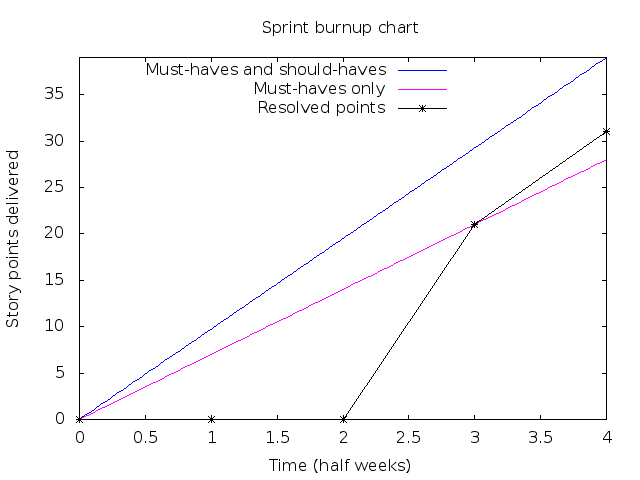
\includegraphics[width=12cm]{img/burnup.png}
	\caption{A burnup graph of our final sprint.}
	\label{fig:burnup}
\end{figure}

Our burnup graph for this sprint can be seen in figure \ref{fig:burnup}. While
it appears as if we are hopelessly behind schedule, please note the following
constraints. Firstly the graph is offset by half a week due to us not meeting up
before then. Secondly this sprint is not done at the time of writing, why we
have some time to complete some more tasks.

Even though we expect to get our round-trip working with the branchy approach
before delivery, as of now, we cannot claim to have reached the goals for this
sprint.

\subsection{Sprint experience}
\label{sec:sprint_experience}
As this was the last sprint of the course -- and thus of the project -- we
wanted to get as many outstanding tasks completed as possible. This resulted in
a very busy sprint log containing almost solely must have tasks. In hindsight
this was a bad move, as we ended up trying to close tasks before they were
actually completed -- a reversal of our previous inability to close completed
tasks -- just to get all tasks done. Our burnup graph (figure \ref{fig:burnup})
partly indicate this, as we have not closed as many tasks as we should.

Since this is a learning project with a parallel development and learning
track, we did not have the option of simply extending the project. Had this been
a pure development project, we would most likely postpone the release date.

We firmly believe that we could not have handled this sprint much differently
from what we did, as the reason for why it got so crowded originates from the
previous sprints, not this one. Taking apart our code was a costly process which
could have been avoided if we had gone for a branchy approach from the very
beginning. An early emphasis on continuous communication with the customer could
have helped this problem. This continuous communication is more in line with
proper SCRUM as well.

Except for the above mentioned issue, this sprint was executed much like our
previous ones. However, the internal roles of the group has become more and more
accentuated over the course of the project -- especially in this sprint and the
last. While we
initially decided not to use and delegate roles for this project, natural roles
have slowly evolved anyway. This is natural for any project involving multiple
people, as people are not all alike, but we did not initially believe it would
be as visible for smaller projects.

\subsection{Sprint learning goal}
\label{sec:sprint_learning_goals}

For this sprint the learning goals entails completing our product and
demonstrating the functionality during class. The slides used for presenting our
product can be found in appendix \ref{sec:presentation_slides}.

As mentioned in section \ref{sec:sprint_goals} we are currently still working on
our product. While the goal for the sprint is to finish as much as possible, we
do not believe that our current status satisfies this.

Having said this, our product was meant partly as a proof of concept. That part
of the project can be considered completed and we are currently working on an
actual implementation of this concept. 

\section{Project retrospective}
\label{sec:project_retrospective}

In this section we will briefly discuss how we worked during the project and the
major points of what worked and what did not.

During this course we developed our product in six iterations. These sprints
were coordinated in collaboration with our customer Praqma and in accordance to
the learning goals set forth by the course. Unfortunately -- due to the nature
of our project and its clear can-it-be-done theme -- the learning goals and
product goals often clashed focus-wise, forcing us to work in two different
directions at the same time. 

Table \ref{tab:sprint_summary} gives an overview of the different sprints and
the goals for each. Notice the difference between the tasks from the product
owner and from the course. Spending time trying to complete both of these at the
same time made some sprints much harder than they should have been and even forced us
to focus on completing either one or the other. 

This could have been avoided through better communication with the project
owners, trying to bend their requirements to the course. However, this is
difficult to do when implementing proof of concept plugins. For example, we
needed a running prototype demonstrating the applicability of the overall idea
where, on the other hand, the software architecture is less important early in
the process (at least in comparison to knowing whether the idea holds).

\begin{table}
	\centering
	\begin{tabular}{| p{2cm} | p{5cm} | p{5cm} |}
		\hline
		Sprint & Product Goal & Course Goal \\
		\hline \hline
		0 & Familiarization with Jenkins and its plugin technology. & Producing
		an architectural protoype implementation. \\
		\hline
		1 & Applying Praqmatic SCRUM to the project. & Applying SCRUM to the
		project. \\
		\hline
		2 & Implementing a primitive round-trip. & Describe the software
		architecture. \\
		\hline
		3 & Getting ready for community release. & Software documentation and
		peer-review of code. \\
		\hline
		4 & Community release and required documentation. & Analyze the
		development process. \\
		\hline
		5 & Finish the project as far as possible & Finish the project as far
		as possible. \\
		\hline
	\end{tabular}
	\caption{Summary of goals for each sprint focusing on the clashes of
	interest between product owner and course requirements.}
	\label{tab:sprint_summary}
\end{table}

Looking back, we should have outlined much earlier in the process when to do
what, instead of taking it all piecemeal sprint by sprint. Especially during the
longer sprints we should have planned more and communicated more with our
product owner, as we made some design decisions he wanted undone when the
sprint was over.

Had we followed proper SCRUM, we would have had weekly meetings and worked on
the project daily which would have helped the problem greatly. However, this is
reserved for full-time jobs and we, as part of a part-time course, did not have
this option. Instead we followed Praqma'a approach which, while based on SCRUM,
adds some flexibility for completion percentage of sprint tasks, allowing us
some leeway. Since we were, and still are, inexperienced with regards to SCRUM,
this approach helped us a lot.

Lastly we all had trouble marking tasks as completed, as there are always more
tests to make, more code to write and more bugs to eradicate. We got better at
this during the course, as we learned to better specify tasks and remind each
other when to stop working on some task. This become apparent when regarding our
burnup graphs for the various sprints, as the amount of tasks completed actually
increase (see appendix \ref{sec:burnup_graphs}).

In conclusion the project and the related development has been intense at times,
both due to the demands of our product owner and due to the split sprint goals.
However, our team worked well together and we had only few serious problems with
our work flow. As such the project work can be labelled a success, even though
the product did not get as far as we hoped and the course material sometimes got
pushed aside to make room for coding sessions.

\newpage
\appendix
\section{Slides from demo presentation}
\label{sec:presentation_slides}
This appendix contains the slides used for presenting our project during the
last lecture of the course.
%Rotate to fit page better
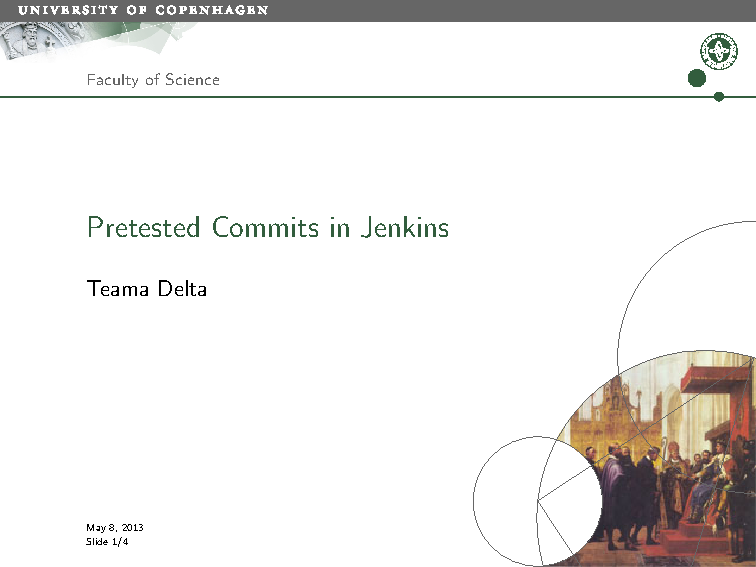
\includepdf[pages=-, angle=90]{aux/presentation.pdf}

\section{Burnup graph collection}
\label{sec:burnup_graphs}
This appendix contains all our burnup graphs, including the just
completed one. Side by side these graphs give an idea of how and when we
developed new strategies or tried new approaches. Please note that the first
sprint (numbered 0) did not include any burnup graph, as it was used for organization and the
second sprint (numbered 1) lacks one, as we tried a textual approach back then.
\begin{figure}[!ht]
	\centering
	\begin{subfigure}[b]{0.4\textwidth}
		\centering
		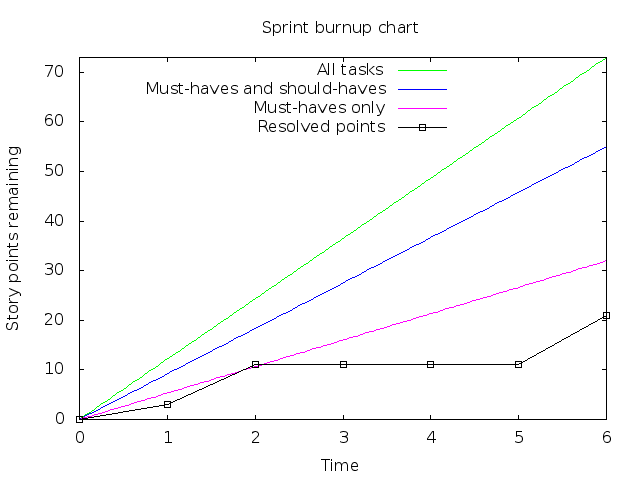
\includegraphics[width=\textwidth]{img/burnup_sprint_3.png}
		\caption{Sprint 2.}
	\end{subfigure}
	\begin{subfigure}[b]{0.4\textwidth}
		\centering
		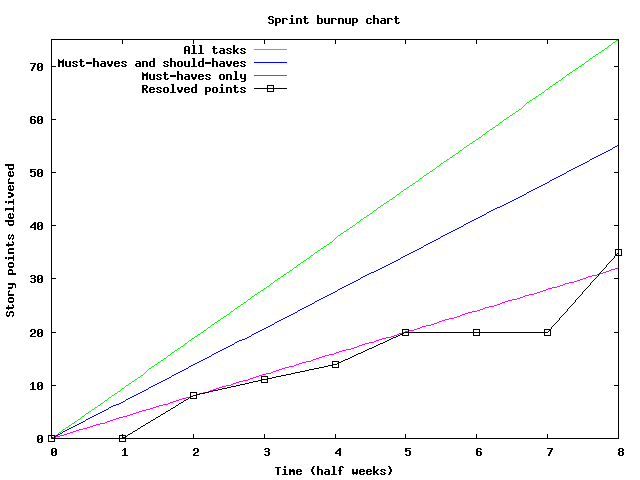
\includegraphics[width=\textwidth]{img/burnup_sprint_4.png}
		\caption{Sprint 3.}
	\end{subfigure}

	\begin{subfigure}[b]{0.4\textwidth}
		\centering
		\centering
		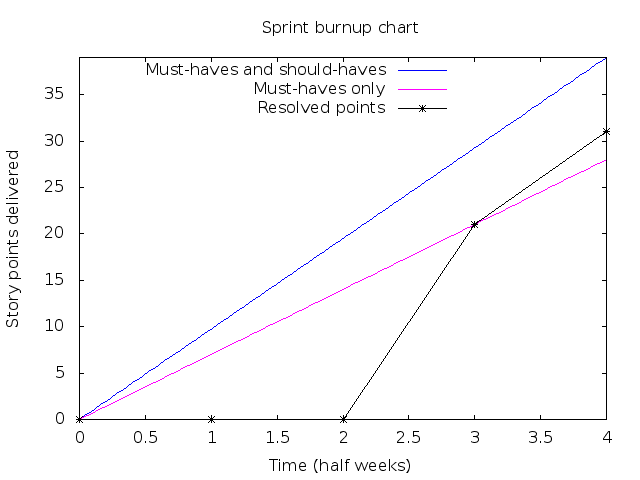
\includegraphics[width=\textwidth]{img/burnup_sprint_5.png}
		\caption{Sprint 4.}
	\end{subfigure}
	\begin{subfigure}[b]{0.4\textwidth}
		\centering
		\centering
		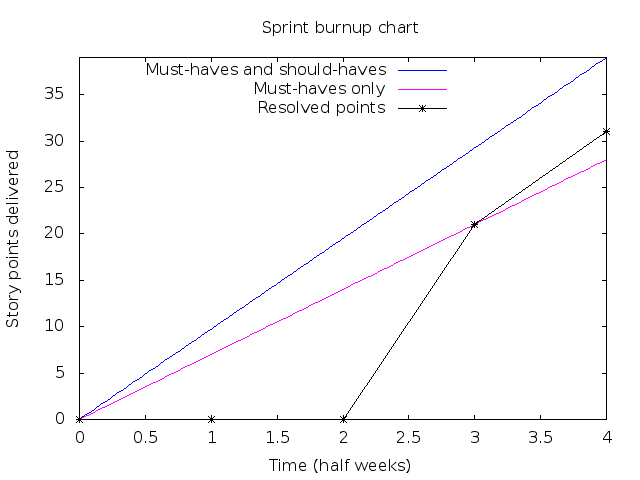
\includegraphics[width=\textwidth]{img/burnup.png}
		\caption{Sprint 5.}
	\end{subfigure}
	\label{Collection of burnup graphs for this Pretested Integration project.}
\end{figure}

\end{document}
